
\section{Seismicity of Northern Iran}

We are interested in applying the visibility graph method to analyze the seismicity of northern Iran. This region is part of the Iranian plateau, on the Himalayan-Alpine seismic belt. It is confined by the relative movements between the Arabian, Eurasian, eastern Asia-Minor, and Indian plates; and has a long history of large magnitude ($M>7$) earthquakes that are well documented dating back to the eight century \citep[e.g.,][]{Berberian_1981_Chap}. According to the tectonic settings and geologic provinces of the plateau, the seismic activity in Iran has been categorized into different seismic zones. These vary between four to nine major seismic zones, in the more traditional models \citep[e.g.,][]{Stocklin1968, Takin1972, Berberian1976}, up to twenty to twenty-three seismotectonic provinces in the most elaborate ones \citep[e.g.,][]{Nowroozi1976, Tavakoli1999}. We adopt the model proposed by \citet{Mirzaei1998} with modifications introduced by \citet{Karimiparidari2013}. In it, Iran is divided into six seismic regions: Azerbaijan, Alborz, Kopeh Dagh, Zagros, Central-East Iran, and Makran. Our focus, however, is on the northern part of Iran, for which we define a region of interest between longitudes 43.5\textdegree{}E and 61.5\textdegree{}E, and latitudes 34\textdegree{}N and 40\textdegree{}N, as shown in Fig.~\ref{fig:study_region}. Although this region encloses part of the Zagros and Central-East seismic zones, we concentrate in the analysis of the seismicity of Azerbaijan, Alborz and Kopeh Dagh.

\begin{figure*}[t]
	\centering
	\includegraphics[width=\textwidth]{figures/pdf/figure-02} 
	\caption{Region of interest, highlighting the seismic zones that are the focus of this study: Azerbaijan, Alborz, and Kopeh-Dagh. The top-right location-map shows Iran and the selected area with respect to neighboring countries. The solid dark lines show the boundaries of the additional Zagros and Central-East seismic zones. This zonation follows the division proposed by \citet{Mirzaei1998} and later modified by \citet{Karimiparidari2013}. The background shows fault lines and the shaded relief. The color version of this figure is available only in the electronic edition.}
	\label{fig:study_region}
\end{figure*}

Northern Iran houses about 41 percent (32 million) of the total population of the country, and has suffered devastating earthquakes in the past \citep[e.g.,][]{Mehrain_1990_Tech, Chafory-Ashtiany_1999_DPM, Razzaghi_2012_Tech}. At the northwest, the seismic zone of Azerbaijan is strongly controlled by the North Tabriz Fault system in the vicinity of the city of Tabriz, shown in Fig.~\ref{fig:study_region}. Historical accounts document the occurrence of strong $M>6$ earthquakes in this region as far back as the ninth century \citep{Berberian1999}, and a few $M>7$ earthquakes in 1042, 1721 and 1780 \citep{Jones1834}. More recently, this region was struck by the $M_w$ 6.1 1997 Ardabil earthquake near the city of Ardabil and the $M_w$ 6.4 2012 Tabriz earthquake northeast of the city of Tabriz. These earthquakes caused extensive damage and took the lives of more than 1,500 people. 

The seismicity in the north-central region of Alborz is dominated by multiple fault systems, including the Talesh, Rubdar, North Alborz, and North Tehran faults, which also have a history of producing strong ground shaking. According to \citet{Ambraseys_1982_Book}, Tehran was devastated by severe $M>7$ earthquakes in 743, 958, 1177, 1665, and 1830. This region has also seen some significant recent seismic activity \citep{Berberian1999}, including the $M_w$ 7.4 1990 Manjil-Rudbar earthquake, which caused numerous deaths and damage to the region in the south Caspian depression, south from the city of Rasht and northwest from Tehran. 

Last, there is the Kopeh Dagh seismic zone to the east and northeast. This region is dominated by the Main Kopeh Dagh Fault system, which exhibits active tectonic displacements along a distance of more than 500 km \citep{Trifonov1978}. This fault is responsible for the $M_w$ 7.3 1948 earthquake, which struck the capital city of Ashgabat in Turkmenistan and destroyed more than 30 villages in Iran. Historically, the Kopeh Dagh seismic zone is also responsible for the $M_s$ 7.1 earthquake in 10 A.D.~\citep{Berberian2001} near Ashgabat, and two significant earthquakes in 1209 and 1405 at the boundary between the Neyshabur and Binalud faults near the city of Mashhad \citep{Berberian1999}.

\begin{figure*}[t]
	\centering
	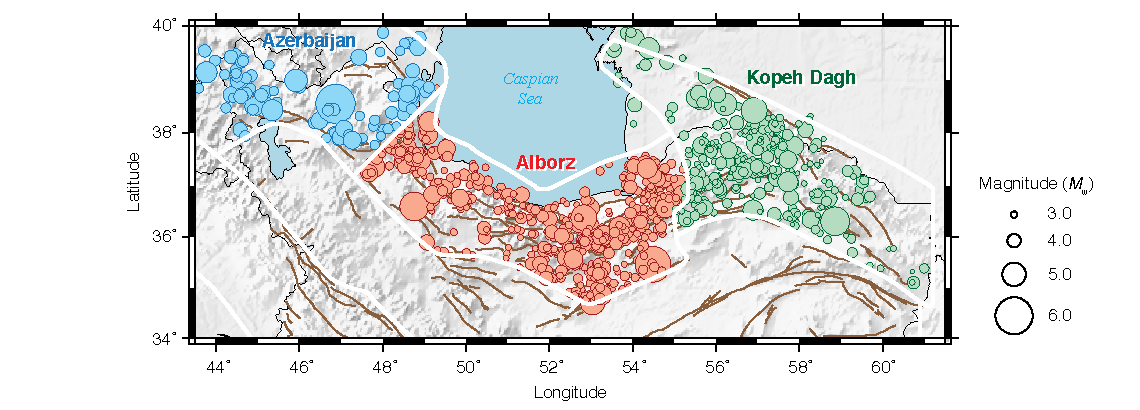
\includegraphics[width=\textwidth]{figures/pdf/figure-03} 
	\caption{Declustered instrumental seismicity of northern Iran for the 2005--2015 period, considering only the events in the seismic zones of interest, namely Azerbaila, Alborz, and Kopeh-Dagh. The size of symbols are proportional to the magnitude of the events, as indicated by the artificial scale shown on the right. The background shows fault lines and the shaded relief. The color version of this figure is available only in the electronic edition.}
	\label{fig:seismicity}
\end{figure*}

It follows from this description that the region of interest is one of significant seismic activity, which goes back centuries. We are, however, interested in the most recent instrumental seismicity. In particular, we focus on events recorded in the last decade, between January 2005 and December 2015. We focus our analysis on this magnitude-time sequence period because in a previous study we observed that the latest decade of seismic records in northern Iran offered the most complete dataset of recorded events, especially for the case of small $M < 4$ earthquakes \citep[e.g.][]{Khoshnevis2016}.

We compiled a catalog of all recorded earthquakes using data downloaded from the International Institute of Earthquake Engineering and Seismology, IIEES (see the Data and Resources section). The obtained dataset contained a mixture of earthquake magnitude scales, including: moment, $M_w$; local, $M_L$; body wave, $m_b$; surface wave, $M_s$; and duration $M_D$ magnitudes. We converted all earthquakes to moment magnitude, $M_w$. Magnitudes in the $M_L$, $m_b$, and $M_s$ scales were converted using the relationships defined in \citet{Zare2014}, whereas $M_D$ magnitudes were converted using the empirical relationship proposed by \citet{Deniz2010}.

Foreshocks and aftershocks were removed from the catalog following a Poissonian occurrence model using the declustering method of \citet{Gardner1974}, in a manner consistent with previous catalog compilations available for the region \citep[e.g.,][]{Zare2014}. Upon declustering, we divide the catalog into three sub-catalogs, each for one of the seismic zones under consideration. Fig.~\ref{fig:seismicity} shows the epicenter location of declustered instrumental earthquakes for the three seismic zones of interest.

We then proceeded to determine the minimum magnitude of completeness, $M_c$, for each region's sub-catalog. The value of $M_c$ is often determined using simple numerical analyses in combination with data inspection. Two common approaches are the maximum curvature (MAXC) and the goodness-of-fit test (GFT) methods \citep{Wiemer2001}. We use the GFT method as introduced by \citet{Wiemer2000}. In this method, the completeness magnitude is obtained such that the catalog satisfies---at a certain acceptance threshold---the Gutenberg-Richter power low, given an extended dataset of events. This extended dataset is composed of predicted and observed events, where the predicted events are generated based on a trial minimum magnitude. The process is repeated for increasing values of the reference minimum magnitude until finding a desirable fit with the power law. \citet{Wiemer2000} suggests a goodness of fit of 90\% as an acceptable threshold to select $M_c$. However, not all frequency-magnitude distributions reach the 90\% mark, in which case $M_c$ can be selected by inspection. 

Figure \ref{fig:completeness} shows the goodness-of-fit values for the three seismic zones. We indicate the selected value of $M_c$ for each region in the figure. We also obtained the $b$-value in the Gutenberg-Richter law for each region following the maximum likelihood estimation \citep{Aki1965}:
% 
\begin{equation}
	b = \frac{log_{10}(e)}{\overline{M} - M_{min}} \, ,
\end{equation}
% 
where $e$ is the mathematical constant or Euler's number, $\overline{M}$ is the average magnitude, and $M_{\min}$ is the minimum magnitude in the sample. Here, the value of $M_{\min}$ is taken as the minimum completeness magnitude $M_c$ obtained or selected for each region's sub-catalog. Table \ref{tab:seismicity} shows the corresponding values of $M_c$ and $b$.

\begin{figure}%[t]
	\centering
	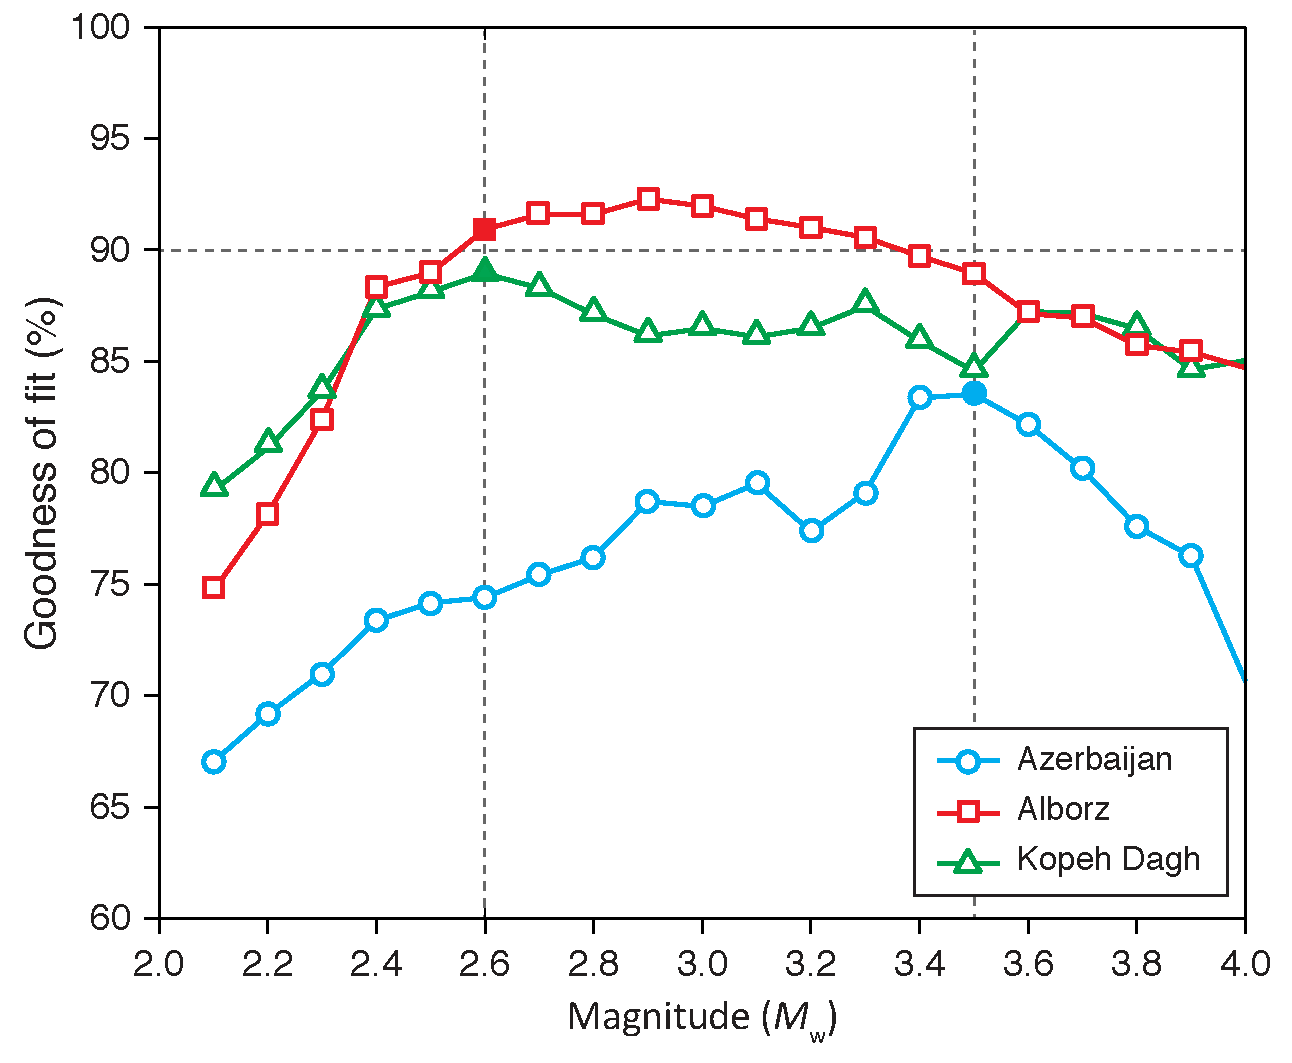
\includegraphics[width=0.45\textwidth]{figures/pdf/figure-04} 
	\caption{Completeness magnitude goodness-of-fit test (GFT) results and selected $M_c$ values for the three tectonic seismic regions in northern Iran as evaluated from the time-magnitude sequence of earthquakes during the 2005--2015 period. The symbols indicate the computed GFT values as function of the earthquake magnitude. The horizontal dashed line indicates the desired threshold for the GFT value at 90 percent. The vertical dashed lines and solid symbols indicate the selected completeness magnitude for each region. The color version of this figure is available only in the electronic edition.}
	\label{fig:completeness}
\end{figure} 

\begin{table}
	\fontfamily{lmss}\selectfont
	\caption{Total and declustered number of earthquakes and seismic parameters $M_c$ and $b$ for the three seismic zones of northern Iran.}
	\centering\small
	\begin{tabular}{|ccccc|}
		\hline
		Region      & Total Num. & Declus.~Num. & \textit{M}c & \textit{b}-value \\ 
		            & of Events  & of Events &             &                  \\
		\hline
		Azerbaijan  &        271 &        93 &         3.5 &             1.02 \\
		Alborz      &       1262 &       794 &         2.6 &             0.77 \\
		Kopeh Dagh  &        399 &       282 &         2.6 &             0.58 \\
		\hline
	\end{tabular}
	\label{tab:seismicity}
\end{table}

\begin{figure*}[t]
	\centering
	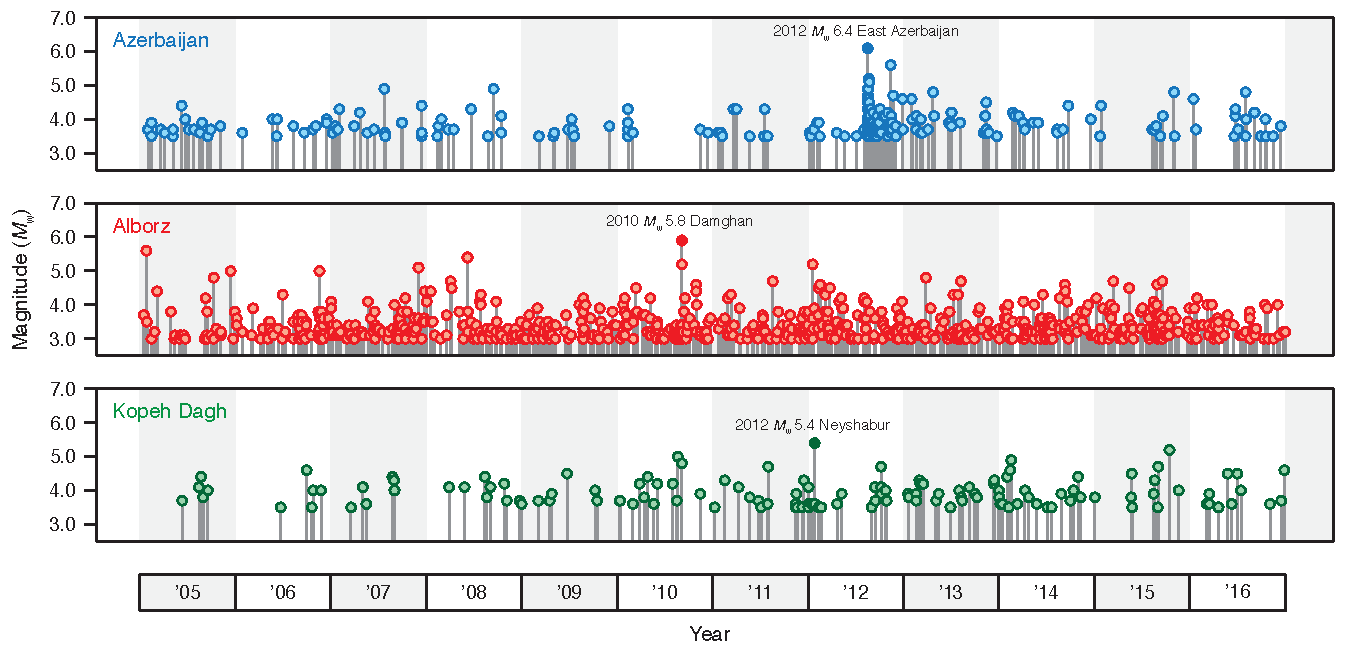
\includegraphics[width=\textwidth]{figures/pdf/figure-05} 
	\caption{Time-magnitude sequences for the northern Iran seismic zones of Azerbaijan, Alborz and Kopeh-Dagh, during the period between 1 January 2005 and 31 December 2015. The event occurrences are represented by vertical bars or sticks of length equal to the $M_w$ magnitude of each earthquake. These sequences correspond to the declustered catalog but in each case we consider only events with $M_w \geq M_c$. As shown in Fig.~\ref{fig:vg}, the dots at the top of each stick represent the nodes of the visibility graphs. The edges or links are omitted for visual convenience. Highlighted in the figure are the largest events in each sub-catalog, namely the 2012 $M_w$ 6.4 East Azerbaijan, 2010 $M_w$ 5.8 Damghan, and 2012 $M_w$ 5.4 Neyshabur earthquakes. The color version of this figure is available only in the electronic edition.}
	\label{fig:mag-time}
\end{figure*}

In addition to using $M_c$ to determine the $b$-value for each sub-catalog, we also use $M_c$ as the threshold for limiting the minimum magnitude to be considered in the construction of the visibility graph of each region. The resulting number of events for each region is included in Table \ref{tab:seismicity}. Figure \ref{fig:mag-time} shows the final time-magnitude sequences for Azerbaijan, Alborz and Kopeh Dagh. Note that in the case of Alborz and Kopeh Dagh, we consider events in the declustered catalog down to $M_w \geq 2.6$, whereas in the case of Azerbaijan all events are $M_w \geq 3.5$.

